% !TEX root = ../agglo_clust_review.tex

\begin{figure}[t]
\centering
% 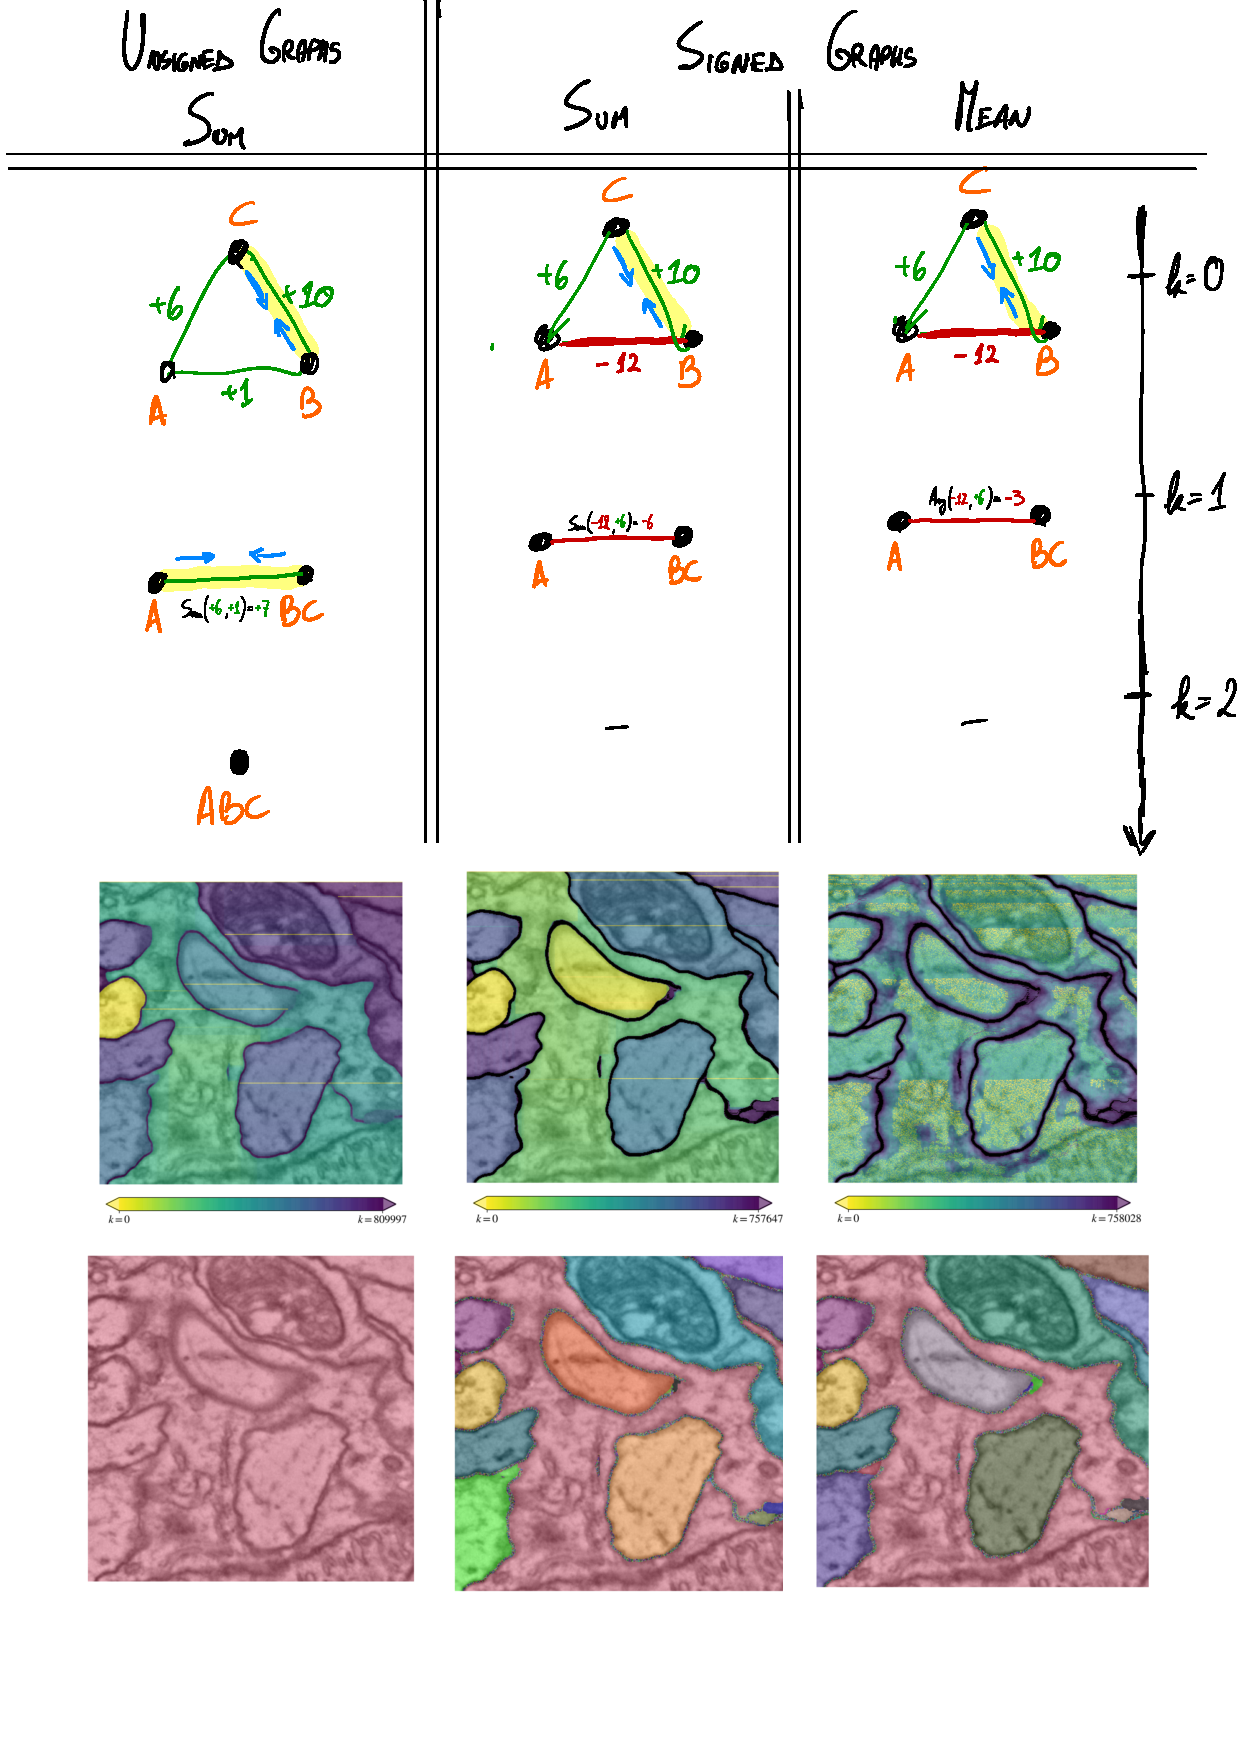
\includegraphics[width=0.5\textwidth,trim=0.4in 1.2in 0.in 0.05in,clip]{./figs/intro_image.jpg} % left bottom right top
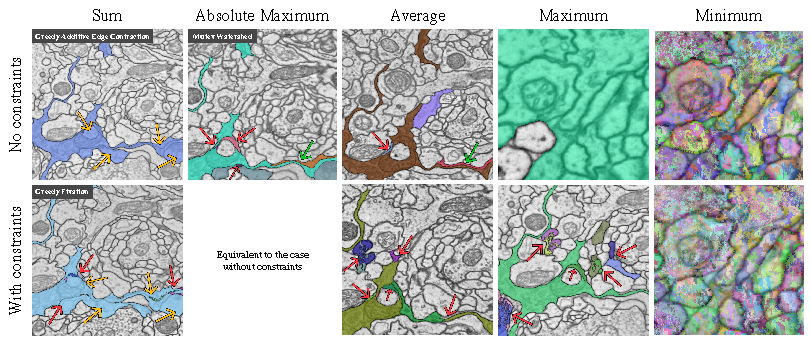
\includegraphics[width=\textwidth]{./figs/comparison.pdf} % left bottom right top
\caption{Failure cases of \algname{} with different linkage criteria highlighted on some difficult parts of the CREMI Challenge \cite{cremiChallenge} training data. Only the few wrongly segmented regions are highlighted in colors. Red arrows point to wrongly split regions. Yellow arrows point out merge errors. Green arrows indicate challenging, but correctly segmented regions. 
% Only the involved segments are colored.
 % main ideas and contributions
\label{fig:cremi_comparison}}
\end{figure}
\begin{figure}
        \centering
\begin{minipage}[T]{0.48\textwidth}
% \begin{table}
    \centering
    \scriptsize
    % \begin{subtable}[t!]{0.5\textwidth}\centering
        \begin{tabular}{l|l|c|c}
        % \toprule
        % & \multicolumn{2}{c}{\thead{Add Cannot-Link Constraints:}} \\
         % & \multicolumn{1}{c}{\thead{\textsc{No}}} & \multicolumn{1}{c}{\thead{\textsc{Yes}}} \\ \midrule
         & \algname{} Linkage & \makecell{Arand} & \makecell{VI-Merge} \\ \midrule
         % & \multicolumn{1}{c}{\thead{$\beta$}}  & \thead{AP} & \multicolumn{1}{c}{\thead{$\beta$}} & \thead{AP} \\ \midrule\midrule
DTWS + LMC \cite{beier2016efficient}& -& & \\
DTWS + avgHC &-& & \\
DTWS  & -& & \\
THRESH &-& & \\ \hline
\algname{} & Average& 0.936 & 0.685 \\
Greedy Fixation \cite{levinkov2017comparative} & Sum + Constr. & 0.906 & 0.642 \\
Mutex Watershed \cite{wolf2018mutex} & Abs. Max.  & 0.897 & 0.714 \\
GAEC \cite{keuper2015efficient} & Sum & 0.872 & 0.539 \\
        \end{tabular}
    \captionof{table}{Arand-Scores and VI-Scores on CREMI challenge training data}
    \label{tab:results_cremi_train}
\end{minipage}\hfill
\begin{minipage}[T]{0.48\textwidth}
    \centering
    \scriptsize
        \begin{tabular}{l|c|c}
         & \makecell{CREMI \\Score} & \makecell{Arand\\Score} \\ \midrule
Our UNet + DTWS + LMC &  \textbf{0.221} & \textbf{0.108}\\
PNI-UNet & 0.228 & 0.116 \\
Our UNet + \algname{} Avg-Linkage & 0.244 & 0.130 \\
MALA-UNet + MC \cite{funke2018large} & 0.276 & 0.132 \\
CRUNet \cite{zeng2017deepem3d} & 0.566 & 0.229 \\
LFC \cite{parag2017anisotropic} & 0.616 & \\
        \end{tabular}
    \captionof{table}{\UPDATE{TBD:} Scores on test data}
    \label{tab:results_cremi_test}
\end{minipage}
\end{figure}

\subsection{CREMI Challenge} \label{sec:cremi_challenge}
We evaluate the algorithms in our framework on the competitive CREMI 2016 EM Segmentation Challenge \cite{cremiChallenge} that is currently the neuron segmentation challenge with the largest amount of training data available. The dataset comes from a serial section EM of \emph{Drosophila} fruit-fly tissue and consists of 6 volumes of 1250x1250x125 voxels at resolution 4x4x40nm, three of which present publicly available training ground truth. The results submitted to the leaderboard are evaluated using the CREMI score\footnote{\url{https://cremi.org/leaderboard/}}, based on the Adapted Rand-Score (Rand-Score) and the Variation of Information Score\cite{arganda2015crowdsourcing}. The data is highly anisotropic and contains artifacts like missing sections, staining precipitations and support film folds. 

\textbf{Training details}
To alleviate difficulties in segmentation, we use a version of the data that was elastically aligned by the challenge organizers with the method \cite{saalfeld2012elastic}.
We train a 3D U-Net \cite{ronneberger2015u, cciccek20163d} using the same architecture as \cite{funke2018large} and predict long-and-short range affinities 
as described in \cite{lee2017superhuman}. In addition to the standard data augmentation techniques of random rotations, random flips and elastic deformations, we simulate data artifacts.
In more detail, we randomly zero-out slices, decrease the contrast of slices, simulate tears, introduce alignment jitter and paste artifacts extracted from the training data. Both \cite{funke2018large} and \cite{lee2017superhuman} have shown
that these kinds of augmentations can help to alleviate issues caused by EM-imaging artifacts.
We use L2 loss and Adam optimizer to train the network.
%\UPDATE{We pre-aligned the training and test data with an elastic alignment method \cite{saalfeld2012elastic}. We further simulated low contrast sections... and missing sections by setting their intensity value to zero... We used 3D U-Net architecture \cite{ronneberger2015u,cciccek20163d} trained with L1 loss (Adam optimizer with learning rate...).} 

\textbf{Additional methods tested }  We compare the performances of the algorithms in our framework with other basic and state-of-the-art post-processing methods. To ensure a fair comparison, we test all methods on the same predictions of our CNN model. As baseline methods, we consider a simple thresholding (THRESH) and a watershed algorithm seeded at the maxima of a boundary distance transform (WSDT). For these baselines, affinities are converted to a boundary map \UPDATE{by taking a weighted average over short- and long-range edge connections}. Other state-of-the-art multi-step-pipelines for neuron-segmentation first find 2D superpixels using WSDT and then apply a graph partitioning algorithm: in our comparison, we include one pipeline using agglomerative HC with average linkage (avgHC) and one using an approximation of the Lifted Multicut Problem (LMC) \cite{beier2016efficient}.


